\documentclass{article}
\usepackage{tikz}
\usetikzlibrary{automata,positioning}

\begin{document}

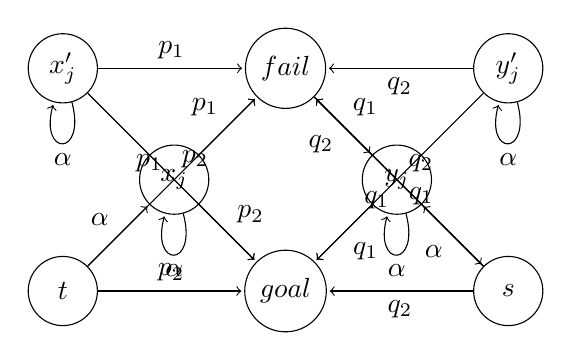
\begin{tikzpicture}[shorten >=1pt,node distance=2cm,on grid,auto]
    \node[state] (x_j) {$x_j$};
    \node[state] (x_j_prime) [above left of=x_j] {$x_j'$};
    \node[state] (t) [below left of=x_j] {$t$};
    \node[state] (goal) [below right of=x_j] {$goal$};
    \node[state] (fail) [above right of=x_j] {$fail$};
    \node[state] (y_j) [below right of=fail] {$y_j$};
    \node[state] (s) [below right of=y_j] {$s$};
    \node[state] (y_j_prime) [above right of=y_j] {$y_j'$};

    \path[->]
        (x_j) edge [loop below] node {$\alpha$} ()
        (x_j) edge node {$p_1$} (fail)
        (x_j) edge node {$p_2$} (goal)
        (x_j_prime) edge [loop below] node {$\alpha$} ()
        (x_j_prime) edge node {$p_1$} (fail)
        (x_j_prime) edge node {$p_2$} (goal)
        (t) edge node {$\alpha$} (x_j)
        (t) edge node {$p_2$} (goal)
        (t) edge node {$p_1$} (fail)
        (fail) edge node {$q_1$} (y_j)
        (fail) edge node {$q_2$} (s)
        (y_j) edge [loop below] node {$\alpha$} ()
        (y_j) edge node {$q_1$} (goal)
        (y_j) edge node {$q_2$} (fail)
        (y_j_prime) edge [loop below] node {$\alpha$} ()
        (y_j_prime) edge node {$q_1$} (goal)
        (y_j_prime) edge node {$q_2$} (fail)
        (s) edge node {$\alpha$} (y_j)
        (s) edge node {$q_2$} (goal)
        (s) edge node {$q_1$} (fail);
\end{tikzpicture}

\end{document}